\documentclass[12pt, landscape, a4paper]{article}
\usepackage[margin=0.5in]{geometry}
\usepackage{tikz}
\usetikzlibrary{positioning, arrows.meta, shapes.multipart, shapes.geometric, calc}
\usepackage{adjustbox}
\usepackage[scaled]{helvet}
\renewcommand\familydefault{\sfdefault}

\begin{document}

% Title Page ===========================
\begin{titlepage}
    \centering
    \vspace*{\fill}
    {\fontsize{50}{60}\selectfont\bfseries ChainVote - ER Diagrams}
    \vspace*{\fill}
\end{titlepage}

\newpage

\section*{1. Chen Notation ER Diagram}
\vspace{1cm}
\begin{center}
\begin{adjustbox}{max width=\textwidth, max height=0.8\textheight}
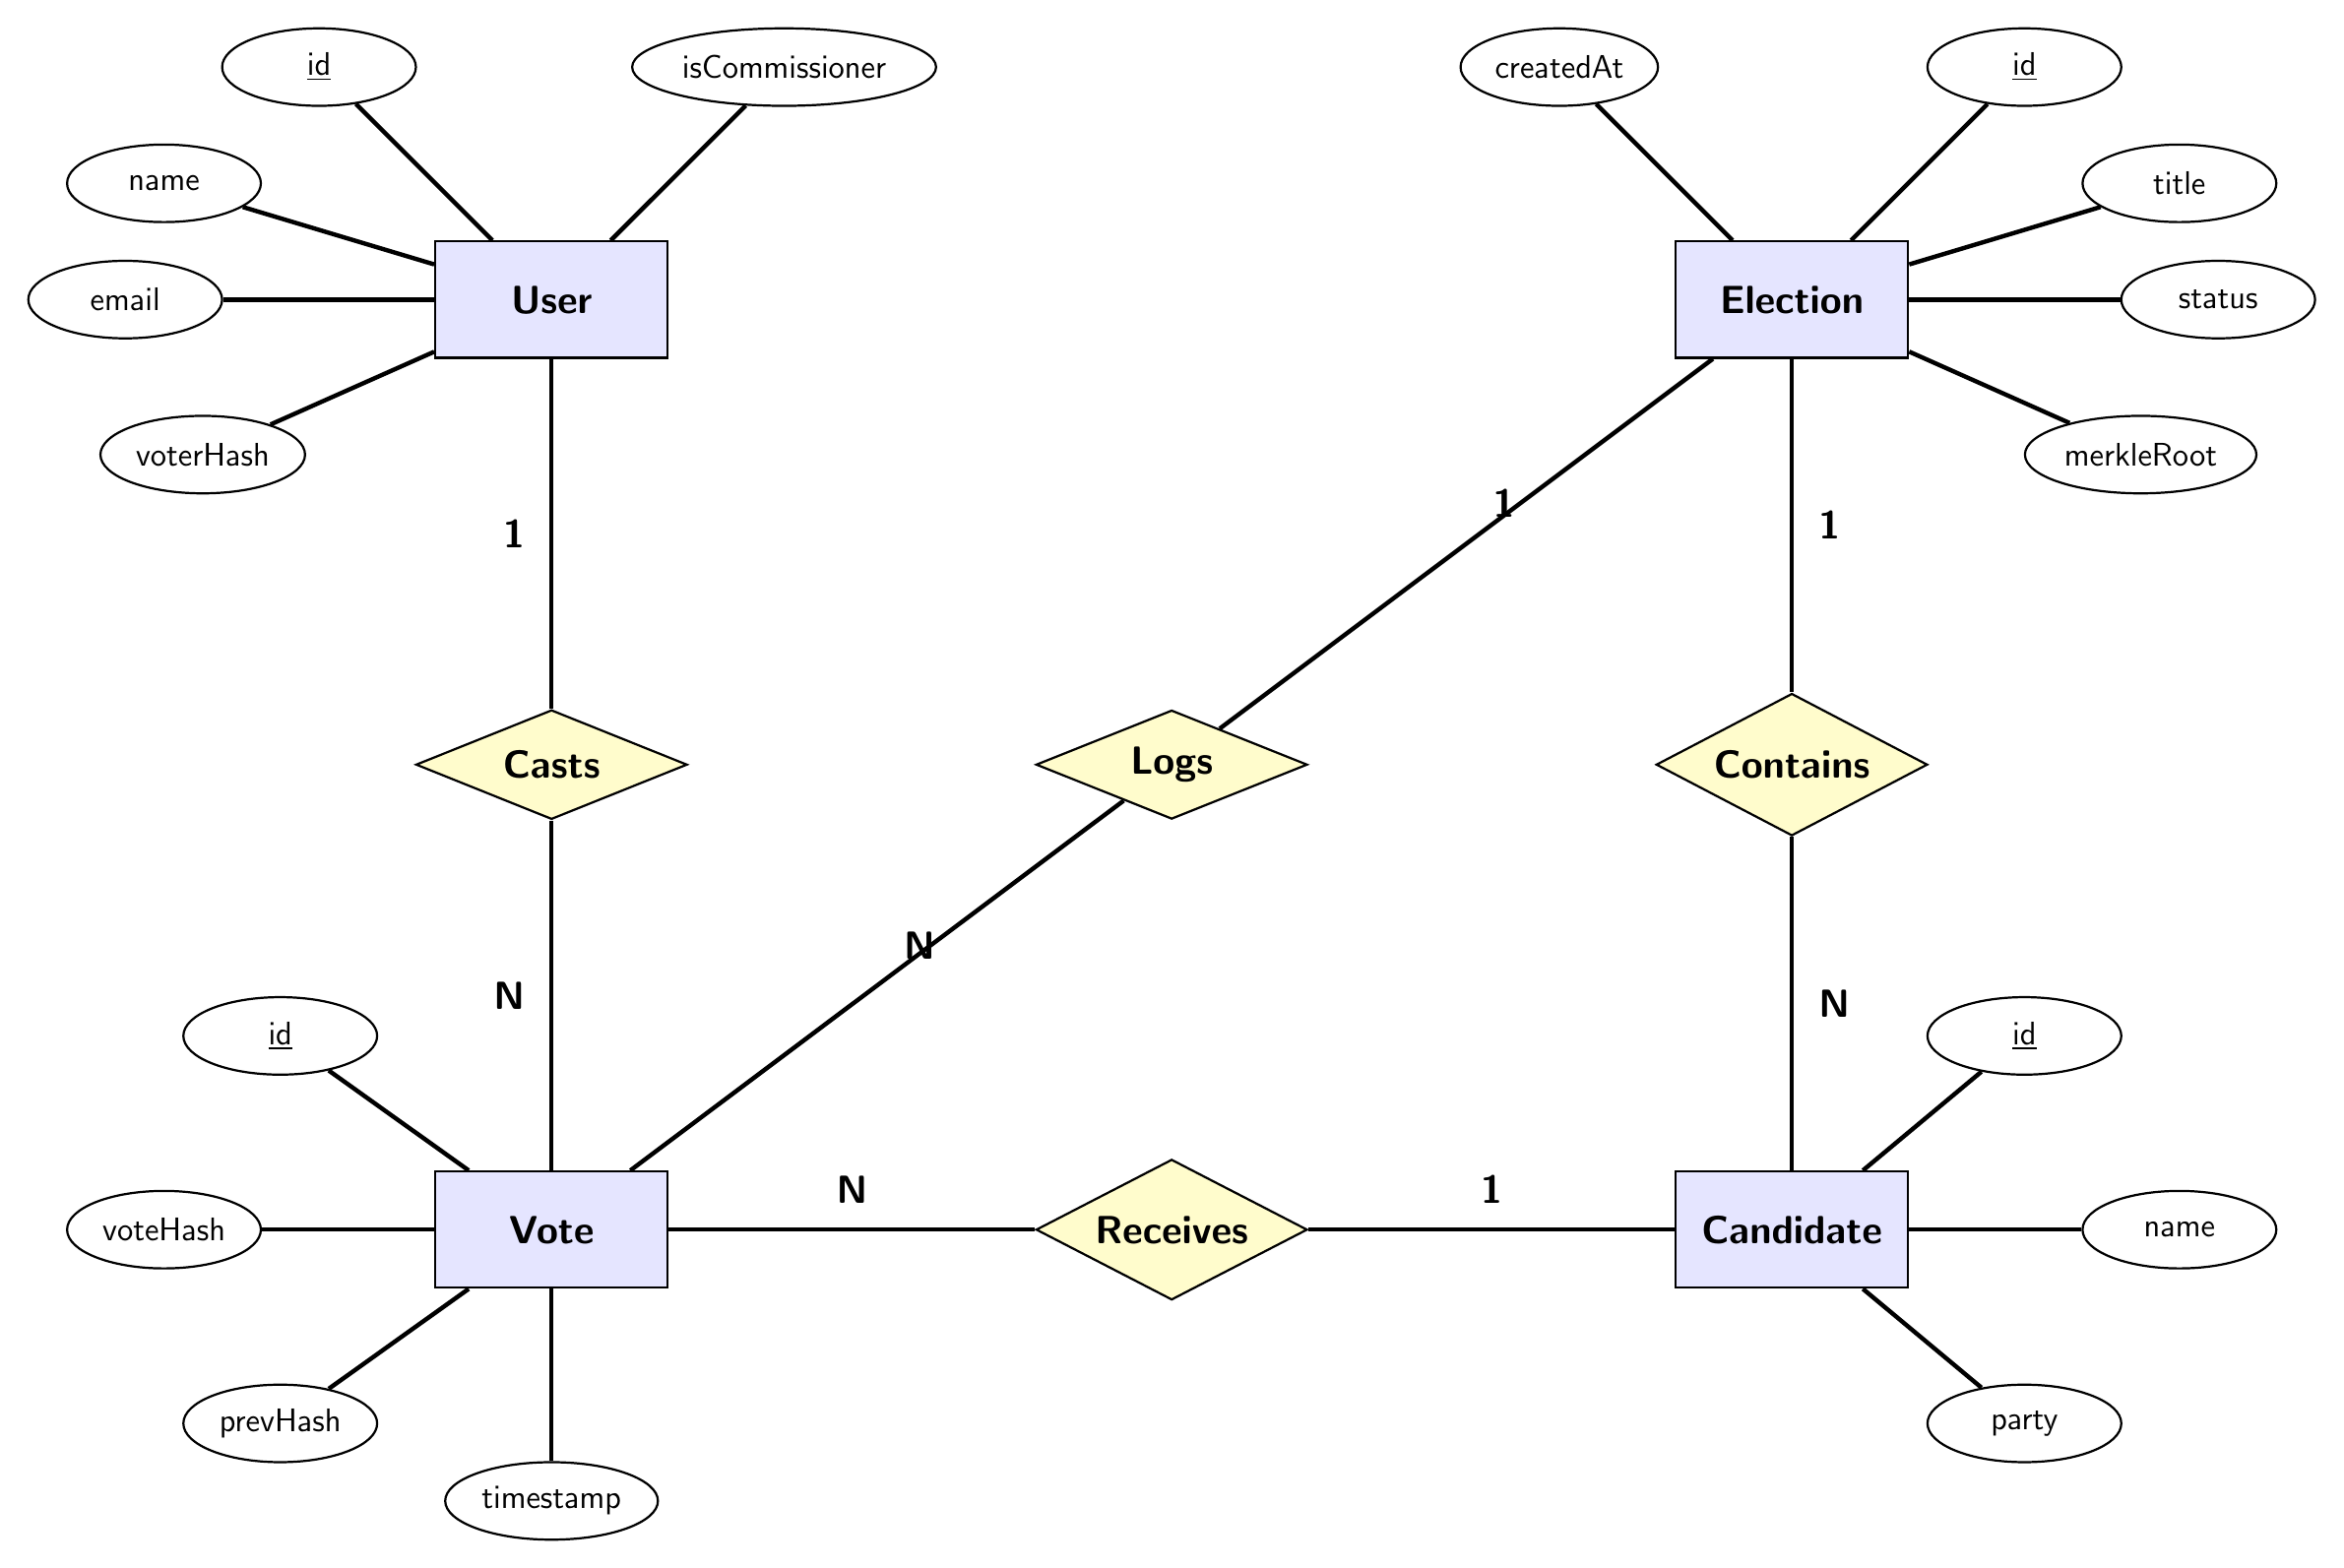
\begin{tikzpicture}[
    entity/.style={rectangle, draw=black, thick, fill=blue!10, minimum width=3cm, minimum height=1.5cm, font=\Large\bfseries},
    attribute/.style={ellipse, draw=black, thick, fill=white, minimum width=2.5cm, minimum height=1cm, inner sep=2pt, align=center, font=\large},
    relationship/.style={diamond, draw=black, thick, fill=yellow!20, aspect=1.8, minimum width=3.5cm, font=\Large\bfseries},
    edge/.style={draw, ultra thick}
]

    % Entities ===========================
    \node[entity] (User) at (0, 0) {User};
    \node[entity] (Election) at (16, 0) {Election};
    \node[entity] (Vote) at (0, -12) {Vote};
    \node[entity] (Candidate) at (16, -12) {Candidate};

    % Relationships ===========================
    \node[relationship] (Casts) at (0, -6) {Casts};
    \node[relationship] (Contains) at (16, -6) {Contains};
    \node[relationship] (Receives) at (8, -12) {Receives};
    \node[relationship] (Logs) at (8, -6) {Logs};

    % Entity <-> Relationship Edges ========
    \draw[edge] (User) -- node[left, font=\Large\bfseries, xshift=-2mm] {1} (Casts);
    \draw[edge] (Casts) -- node[left, font=\Large\bfseries, xshift=-2mm] {N} (Vote);
    
    \draw[edge] (Election) -- node[right, font=\Large\bfseries, xshift=2mm] {1} (Contains);
    \draw[edge] (Contains) -- node[right, font=\Large\bfseries, xshift=2mm] {N} (Candidate);
    
    \draw[edge] (Candidate) -- node[above, font=\Large\bfseries, yshift=2mm] {1} (Receives);
    \draw[edge] (Receives) -- node[above, font=\Large\bfseries, yshift=2mm] {N} (Vote);
    
    \draw[edge] (Election) -- node[above right, font=\Large\bfseries, xshift=2mm, yshift=2mm] {1} (Logs);
    \draw[edge] (Logs) -- node[above right, font=\Large\bfseries, xshift=2mm, yshift=2mm] {N} (Vote);

    % User Attributes ===========================
    \node[attribute] (uid) at (-3, 3) {\underline{id}};
    \node[attribute] (uname) at (-5, 1.5) {name};
    \node[attribute] (uemail) at (-5.5, 0) {email};
    \node[attribute] (uvoter) at (-4.5, -2) {voterHash};
    \node[attribute] (ucom) at (3, 3) {isCommissioner};
    
    \draw[edge] (User) -- (uid);
    \draw[edge] (User) -- (uname);
    \draw[edge] (User) -- (uemail);
    \draw[edge] (User) -- (uvoter);
    \draw[edge] (User) -- (ucom);

    % Election Attributes ===========================
    \node[attribute] (eid) at (19, 3) {\underline{id}};
    \node[attribute] (etitle) at (21, 1.5) {title};
    \node[attribute] (estatus) at (21.5, 0) {status};
    \node[attribute] (emerkle) at (20.5, -2) {merkleRoot};
    \node[attribute] (ecreate) at (13, 3) {createdAt};
    
    \draw[edge] (Election) -- (eid);
    \draw[edge] (Election) -- (etitle);
    \draw[edge] (Election) -- (estatus);
    \draw[edge] (Election) -- (emerkle);
    \draw[edge] (Election) -- (ecreate);

    % Candidate Attributes ===========================
    \node[attribute] (cid) at (19, -9.5) {\underline{id}};
    \node[attribute] (cname) at (21, -12) {name};
    \node[attribute] (cparty) at (19, -14.5) {party};
    
    \draw[edge] (Candidate) -- (cid);
    \draw[edge] (Candidate) -- (cname);
    \draw[edge] (Candidate) -- (cparty);

    % Vote Attributes ===========================
    \node[attribute] (vid) at (-3.5, -9.5) {\underline{id}};
    \node[attribute] (vhash) at (-5, -12) {voteHash};
    \node[attribute] (vprev) at (-3.5, -14.5) {prevHash};
    \node[attribute] (vtime) at (0, -15.5) {timestamp};
    
    \draw[edge] (Vote) -- (vid);
    \draw[edge] (Vote) -- (vhash);
    \draw[edge] (Vote) -- (vprev);
    \draw[edge] (Vote) -- (vtime);

\end{tikzpicture}
\end{adjustbox}
\end{center}

\newpage
\section*{2. Crow's Foot Notation Diagram}
\vspace{2cm}
\begin{center}
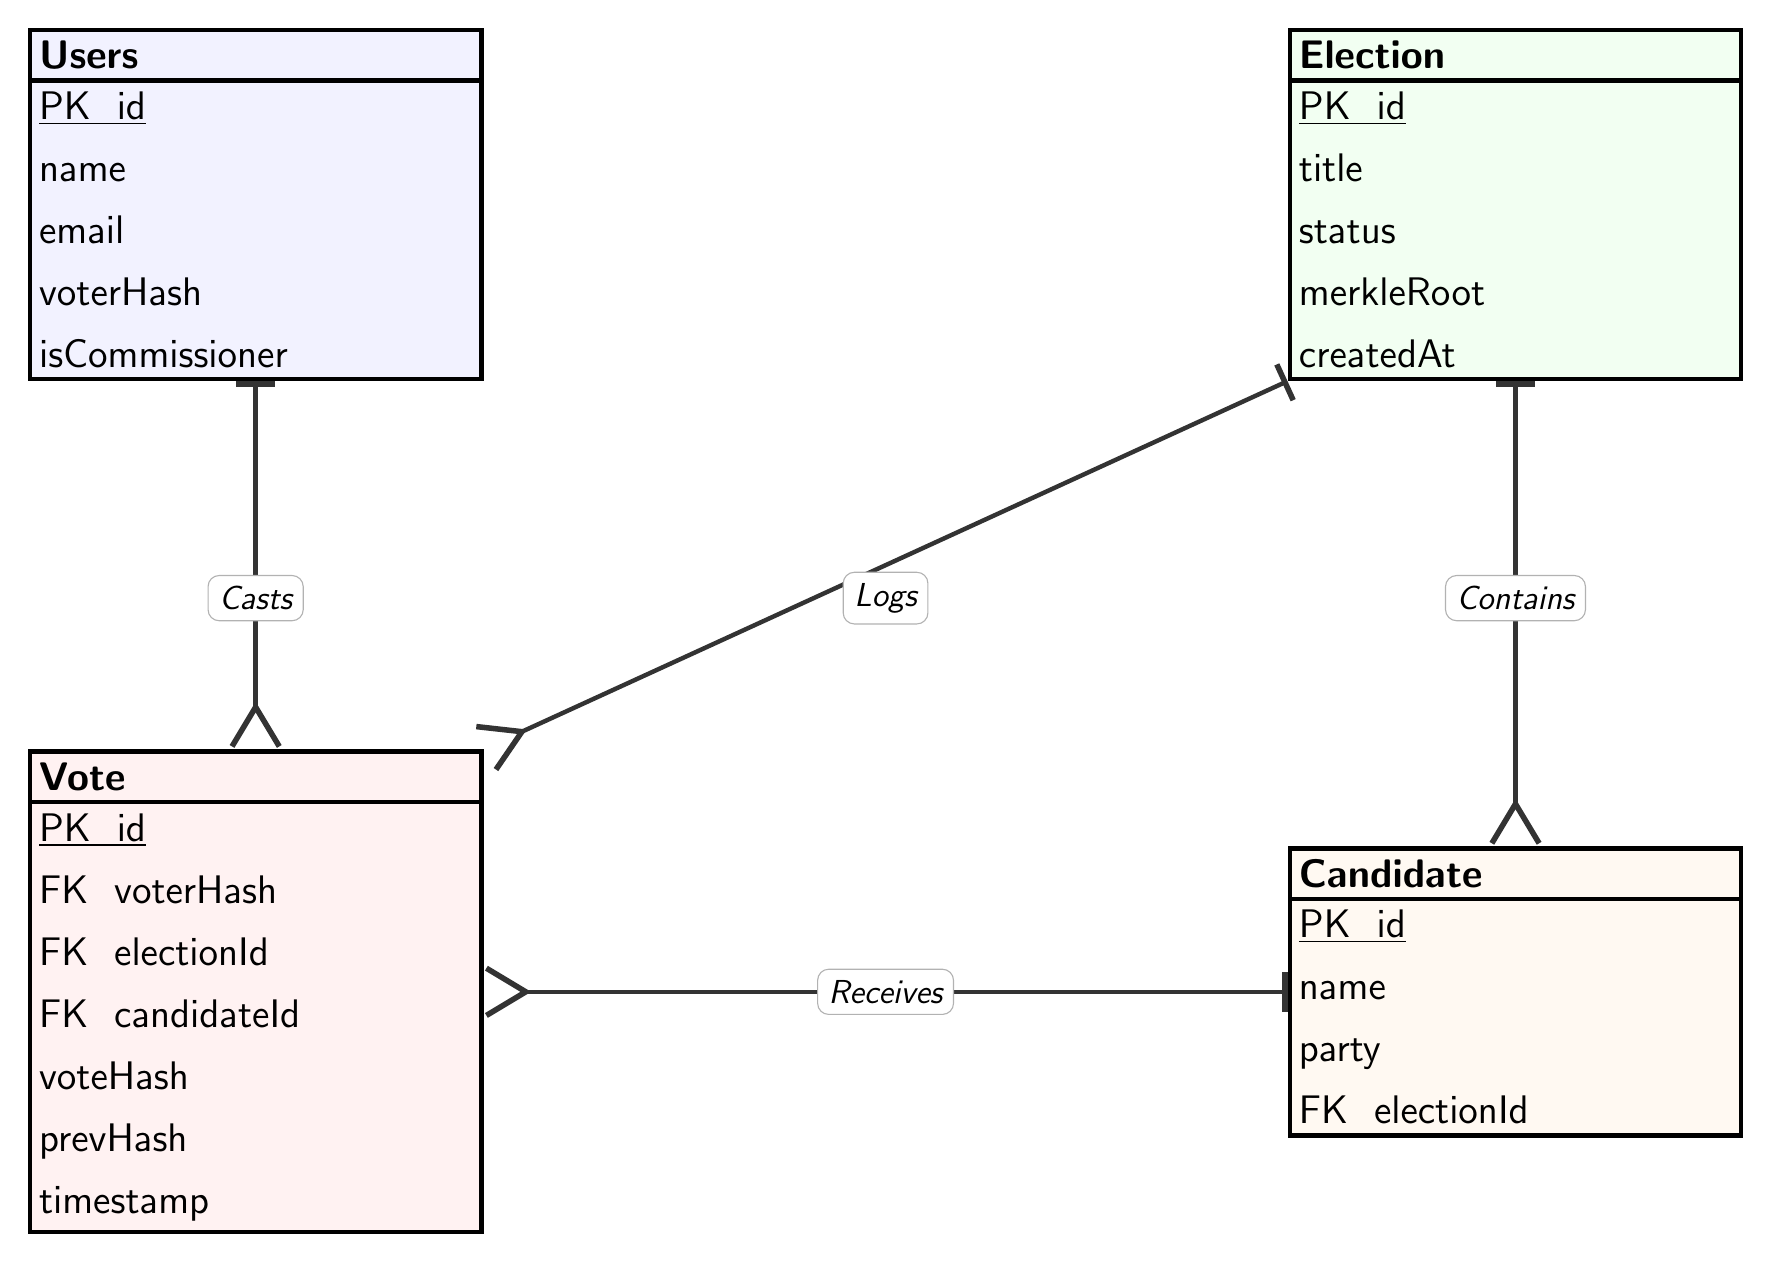
\begin{tikzpicture}[
    table/.style={
        rectangle split,
        rectangle split parts=2,
        draw, ultra thick,
        text width=5.5cm,
        font=\fontsize{14}{16}\selectfont
    },
    crowsfoot/.style={
        ultra thick,
        {Bar[width=5mm, line width=2pt]}-{Straight Barb[length=5mm, width=6mm, reversed, line width=2pt]},
        draw=black!80
    }
]

    % The 4 Tables ===========================
    \node[table, fill=blue!5, rectangle split part fill={blue!20, white}] (User) at (0, 0) {
        \textbf{Users} 
        \nodepart{second}
        \underline{PK \ id} \\[1ex]
        name\\[1ex]
        email\\[1ex]
        voterHash\\[1ex]
        isCommissioner
    };

    \node[table, fill=green!5, rectangle split part fill={green!20, white}] (Election) at (16, 0) {
        \textbf{Election} 
        \nodepart{second}
        \underline{PK \ id} \\[1ex]
        title\\[1ex]
        status\\[1ex]
        merkleRoot\\[1ex]
        createdAt
    };

    \node[table, fill=orange!5, rectangle split part fill={orange!20, white}] (Candidate) at (16, -10) {
        \textbf{Candidate} 
        \nodepart{second}
        \underline{PK \ id} \\[1ex]
        name\\[1ex]
        party\\[1ex]
        FK \ electionId
    };

    \node[table, fill=red!5, rectangle split part fill={red!20, white}] (Vote) at (0, -10) {
        \textbf{Vote} 
        \nodepart{second}
        \underline{PK \ id} \\[1ex]
        FK \ voterHash\\[1ex]
        FK \ electionId\\[1ex]
        FK \ candidateId\\[1ex]
        voteHash\\[1ex]
        prevHash\\[1ex]
        timestamp
    };

    % Crow's Foot Connection Edges ====================
    % From User to Vote (1 to N)
    \draw[crowsfoot] (User.south) -- (Vote.north);
    
    % From Election to Candidate (1 to N)
    \draw[crowsfoot] (Election.south) -- (Candidate.north);
    
    % From Candidate to Vote (1 to N)
    \draw[crowsfoot] (Candidate.west) -- (Vote.east);
    
    % From Election to Vote (1 to N)
    \draw[crowsfoot] (Election.south west) -- (Vote.north east);

    % Informational Labels floating above the lines ==================
    \node[fill=white, inner sep=4pt, font=\large\itshape, draw=black!30, rounded corners] at (0,-5) {Casts};
    \node[fill=white, inner sep=4pt, font=\large\itshape, draw=black!30, rounded corners] at (16,-5) {Contains};
    \node[fill=white, inner sep=4pt, font=\large\itshape, draw=black!30, rounded corners] at (8,-10) {Receives};
    \node[fill=white, inner sep=4pt, font=\large\itshape, draw=black!30, rounded corners] at (8,-5) {Logs};

\end{tikzpicture}
\end{center}

\end{document}